  \documentclass[a4paper,
fontsize=11pt,
%headings=small,
oneside,
numbers=noperiodatend,
parskip=half-,
bibliography=totoc,
final
]{scrartcl}

\usepackage{synttree}
\usepackage{graphicx}
\setkeys{Gin}{width=.4\textwidth} %default pics size

\graphicspath{{./plots/}}
\usepackage[ngerman]{babel}
\usepackage[T1]{fontenc}
%\usepackage{amsmath}
\usepackage[utf8x]{inputenc}
\usepackage [hyphens]{url}
\usepackage{booktabs} 
\usepackage[left=2.4cm,right=2.4cm,top=2.3cm,bottom=2cm,includeheadfoot]{geometry}
\usepackage{eurosym}
\usepackage{multirow}
\usepackage[ngerman]{varioref}
\setcapindent{1em}
\renewcommand{\labelitemi}{--}
\usepackage{paralist}
\usepackage{pdfpages}
\usepackage{lscape}
\usepackage{float}
\usepackage{acronym}
\usepackage{eurosym}
\usepackage[babel]{csquotes}
\usepackage{longtable,lscape}
\usepackage{mathpazo}
\usepackage[normalem]{ulem} %emphasize weiterhin kursiv
\usepackage[flushmargin,ragged]{footmisc} % left align footnote
\usepackage{ccicons} 

\usepackage{listings}

\urlstyle{same}  % don't use monospace font for urls

\usepackage[fleqn]{amsmath}

%adjust fontsize for part

\usepackage{sectsty}
\partfont{\large}

%Das BibTeX-Zeichen mit \BibTeX setzen:
\def\symbol#1{\char #1\relax}
\def\bsl{{\tt\symbol{'134}}}
\def\BibTeX{{\rm B\kern-.05em{\sc i\kern-.025em b}\kern-.08em
    T\kern-.1667em\lower.7ex\hbox{E}\kern-.125emX}}

\usepackage{fancyhdr}
\fancyhf{}
\pagestyle{fancyplain}
\fancyhead[R]{\thepage}

%meta
%meta

\fancyhead[L]{B. Kaden \\ %author
LIBREAS. Library Ideas, 31 (2017). % journal, issue, volume.
\href{http://nbn-resolving.de/
}{}} % urn
\fancyhead[R]{\thepage} %page number
\fancyfoot[L] {\ccLogo \ccAttribution\ \href{https://creativecommons.org/licenses/by/3.0/}{\color{black}Creative Commons BY 3.0}}  %licence
\fancyfoot[R] {ISSN: 1860-7950}

\title{\LARGE{Shoebox Science Kits und 155 weitere Bibliotheksideen aus dem Jahr 1977}} %title %title
\author{Ben Kaden} %author

\setcounter{page}{1}

\usepackage[colorlinks, linkcolor=black,citecolor=black, urlcolor=blue,
breaklinks= true]{hyperref}

\date{}
\begin{document}

\maketitle
\thispagestyle{fancyplain} 

%abstracts

%body
Ganze elf Jahre und einiges an Zufällen brauchte es, bis wir von
LIBREAS. Library Ideas unsere Vorgängerpublikation entdecken konnten.
Dabei weist der Worldcat Dale E. Shaffers 1977 im Eigenverlag
erschienene Handreichung \emph{A Handbook of Library Ideas} als Original
sogar in zwei Bibliotheken nach: in der British Library und in der
Harold B. Lee Library der Brigham Young University. Ein weiteres
Exemplar gibt es in jedem Fall in im Harold Washington Library Center
der Chicago Public Library, denn dieses ist der Glücksfund, welcher uns
wiederum eine Ausgabe auf den Schreibtisch bringt. Dort fand nämlich
Marc Fisher, Initiator und Betreiber der wunderbaren
Ephemera-Sammelstelle PUBLIC COLLECTORS (siehe
\href{http://www.publiccollectors.org}{\emph{www.publiccollectors.org}})
ein Exemplar und publizierte es pünktlich zum 40. Jahrestages seines
Erscheinens als Reprint in seiner Reihe \enquote{Library Excavations}.

I

Der 2009 verstorbene Dale Eugene Shaffer erhielt dadurch zugleich eine
Art postume Würdigung. Während seiner Karriere hatte er sich auf das
Beraten von Bibliotheken spezialisiert, was sich heute vor allem in
seiner eindrucksvollen Publikationsliste zeigt, die außerdem noch mehr
als zwei Dutzend Bücher Regionalgeschichte zu seiner Heimatstadt Salem,
Ohio umfasst. Begonnen hatte die akademische Laufbahn des am
17.~April~1929 in eben diesem Salem geborenen Dale E. Shaffer mit einem
Bachelor in Betriebswirtschaft, den er um einen Master in Library
Science an der Kent State University ergänzte. Weiter ging es zunächst
in einem erwerbsbiografischen Patchwork-Modus, wie man ihn auch heute
mit einem Abschluss in Bibliothekswissenschaft gut kennt: ein Jahr
(1956--1957) bei General Electric, danach Dozent für Wirtschaft am
Bethany College in West Virginia, ab 1960 ein Jahr Technical Research
Librarian in der Schulverwaltung von South Bend, Indiana. Im frühen 1963
begann er als Bibliothekar des Glenville State College in West Virginia,
wie die Ausgabe der College-Zeitung Glenville Mercury vom 13.02.1963 auf
der Titelseite unter einer Bildleiste zur Wahl des Campus Cover Girl
berichtete und außerdem alle Beteiligten auflistete, die ihn bei
Reorganisation und Betrieb der Bibliothek unterstützten und die hier
ruhig mal für eine Sekunde kurzen Aufschimmerns aus dem Schatten der
Vergangenheit geholt werden können:

\begin{quote}
\enquote{Thirteen students are working in the library during second
semester. David Gillespie, Janice Underwood, Marie Jewell, Helen
Cunningham, Sandy Williams, Louis Friel and Greta James work at the
circulation desk. Virginia Gallaher is typist and Carl Paxton helps with
the processing of books. Ron Hill and Paul Taylor do general work.
Mrs.~Dorothy Peterson is assistant librarian and Miss Mary Susan Brown
is in charge of circulation.} (Janet Long: GSC Librarian begins Work.
IN: The Glenville Mercury, 13.02.1963, S. 1/4)
\end{quote}

Dies also als kurzer Einblick in die Personalausstattung einer
US-College Bibliothek der 1960er Jahre. Nicht viel später wechselte Dale
E. Shaffer zur Capital University in Columbus, Ohio und organisierte
selbige ebenfalls gründlich um und neu. Später baute er das
Bibliothekssystem des neu gegründeten Ocean County College in Toms
River, New Jersey auf. Im Jahr 1968 veröffentlichte er unter dem schönen
Titel \emph{The maturity of librarianship as a profession} (Metuchen,
N.~J. : Scarecrow Press) das erste von zahlreichen Büchern, in denen er
seine Erfahrungen zur Bibliotheksentwicklung aufarbeitete. In seinem
Erstling legte er vor allem dar, dass die Bibliotheksarbeit zwar eine
Reihe von spezifischen Fertigkeiten und Anforderungen mit sich bringt,
jedoch noch keinesfalls den Reifegrad erreicht hat, den ein
Tätigkeitsfeld benötigt, damit man von einem Beruf beziehungsweise einer
Profession sprechen kann. Nach dem in seinem Ansatz verfolgten
Entwicklungsmodell war das Bibliothekswesen erst in der Präadoleszenz.
Das setzte schon ein gewisses Ausrufezeichen, vor allem in der
nordamerikanischen Bibliothekswelt, und bereitete den Weg für sein
weiteres Beratungs- und Publikationsprogramm.

\begin{figure}
\centering
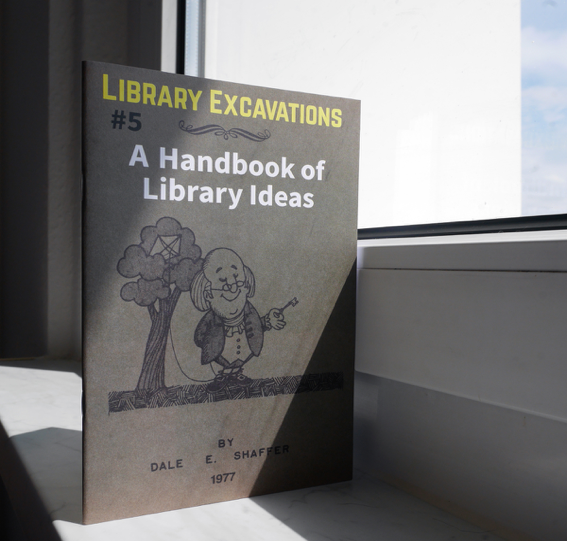
\includegraphics{lib_excavations.png}
\caption{}
\end{figure}

II

Mit seinen Bemühungen zur Evaluierbarkeit des Professionalisierungsgrads
der Bibliotheksarbeit muss sich glücklicherweise nicht beschäftigen, wer
nur in der schmalen Nebenpublikation zu den Library Ideas blättert.
Diese wirkt so freundlich wie spleenig und verzeichnet, so das Vorwort,
einige tatsächlich beobachtete \enquote{novel and non-traditional
approaches}. Handlungsanleitungen liefert der Autor nicht, sondern
bewusst nur \enquote{sufficient information to trigger action}. Zugleich
würdigt, fast feiert er \enquote{creative librarians}, also diejenigen,
welche, wie man heute phrasieren würde, \enquote{out of the box} zu
denken fähig sind. Konsequenterweise eröffnet er mit den
Grundanforderungen an, so eine ad-hoc-Übersetzung,
Kreativbibliothekar\_innen. Zwölf sind es, von grundsätzlicher Neugier,
Willen zur Vorstellungskraft, Sensibilität, Abstraktionsvermögen,
Unabhängigkeit, Ausdauer und Mut. Interessant und als schöne Variation
zu stereotypen Vorstellungen ist der Punkt Nummer~9 -- Challenged by
Disorder:

\begin{quote}
\enquote{He {[}der Kreativbibliothekar{]} thrives on chaos and
disorganization, considering it a problem to be solved.}
\end{quote}

Die Unordnung ist das Material, an dem sich die Ordnungskraft entfaltet.

Die 156 Ideen in alphabetischen Folge zeigen heute unter anderem
eindrücklich, wie alt all das ist, was heute unter dem Label Makerspaces
diskutiert wird. Genau genommen ist der Grundansatz noch deutlich älter,
wie man bei der Idee Nummer 140 -- Tool-Lending Pool -- lernt:

\begin{quote}
\enquote{Tool lending was originally established by Rotarians during the
shortages of World War II. Now, power tools can be borrowed from some
libraries for three days; hand tools for a week. Included are
tachometersm strobe lights, and various items for automobile tuneups.}
(S.~35)
\end{quote}

Und plötzlich erkennt man, dass auch Baumärkte und Bibliotheken ihr
Serviceprofil einander annähern können.

Für Zoohandlungen gilt dies hoffentlich nicht und man wünscht sich, dass
Beispiel \enquote{Animal Lending} (\enquote{Libraries now loan small,
caged animals free of charge for one or two weeks.}, 3) für immer perdu
ist. Baby Welcome Cards (7), die man oft von Fußball-Fanclubs kennt,
gibt es dagegen hier und da. Die Idee wurde sogar, wie eine
Google-Recherche sofort offenbart, auch schon mal zum Welcome Baby
Brunch erweitert.

Manches aus dem Ideenpool wirkt naturgemäß reichlich antiquiert oder
abseitig, beispielsweise die Idee, Standwaagen einzuführen
(\enquote{Weight control is of convenient way for students to keep track
of it.}, 9), auch wenn man sich nicht ohne Melancholie daran erinnert,
wie die Münz-Personen-Waagen im Berliner U-Bahnsystem mit dem
unermüdlichen Rentner, der sie lange über ihre öffentliche Notwendigkeit
hinaus pflegte und betrieb, 2011 verschwanden.\footnote{Mehr zu diesem
  Thema:
  \href{http://www.tagesspiegel.de/berlin/stadtleben/ausgewogen-das-ende-der-u-bahn-waagen/4411630.html}{\emph{http://www.tagesspiegel.de/berlin/stadtleben/ausgewogen-das-ende-der-u-bahn-waagen/4411630.html}}}

Das zur Gewichtsprüfkultur gegenläufige Programm verbirgt sich hinter
einem \enquote{Hamburgers for Overdues}-Programm (59):

\begin{quote}
\enquote{Rather than spend money on mailing overdue notices to patrons,
one library is offering free hamburger coupons to those who return
library materials. It is done in cooperation with a large
fast-food-chain, which also tends to benefit from the idea.
{[}\ldots{}{]} For promotional purposes, the food chain also offers free
hamburgers to children who fulfill the library's summer reading
requirements.}
\end{quote}

Auch abgesehen davon, dass dieses Programm vegetarischen und veganen
Ernährungsmodellen wenig Rechnung trägt, wirkt der
\enquote{Lies-Dich-Dick}-Ansatz nicht ganz ausgereift. Aber als
Grundidee für gesundheitsfördende oder -neutrale Goodies kann man diese
Public-Private-PR-Partnerschaft möglicherweise sogar etwas länger
bedenken.

Bedenkenswert ist bei anderen Programmen vor allem die Bezeichnung:
\enquote{Books for Crooks} (16) klingt heute eher wie eine, mäßige,
Saturday-Night-Live-Sketch-Idee und wenn man dazu liest, wie der Scope
über Gefangenbüchereien ausgedehnt wurde, wird es noch befremdlicher:
\enquote{Bookracks were even set up in taverns.} Das heutige Pendant zu
dieser Art Outreach wäre per Klischee wahrscheinlich der Gang zu einem
Ort für \enquote{Internationale Sportwetten.} In vielen gastronomischen
Lokalen in Berlin wie unter anderem der sehr passend benannten Böse
Buben Bar sammeln sich dagegen Bücher auch ohne Zutun der Öffentlichen
Bibliotheken und zwar erfahrungsgemäß in deutlich größerer Anzahl als
die Angehörigen des Gangsterwesens.

Unter dieser Buch-und-Schnaps-Idee findet sich dagegen etwas mit sogar
wachsendem Potential erwähnt: \enquote{Books with Meals-on-Wheels} (17),
was genau das besagt, was der Name sagt: Bibliotheksbücher werden mit
dem Essen auf Rädern ausgeliefert und abgeholt. Für alternde
Gesellschaften ist das durchaus überlegenswert. Ähnliches findet sich
unter Idee 63 -- Home-Bound-Library-Delivery -- und man sollte bei der
Gelegenheit anmerken, dass angesichts der demografischen Entwicklung
bestimmte Formen der Sozialen Bibliotheksarbeit keineswegs als überholt
gelten müssen -- oder sollten (siehe auch Idee 105 -- Nursing home
library).

Erwartungsgemäß kann man an der Ideensammlung schließlich Formen des
Medienwandels gut nachvollziehen und sowohl als Avantgarde wie auch als
Sackgasse. Sehr wegweisend wirkt die Idee Nummer~30 namens Computerized
Book Circulation, die ein vernetztes System zwischen Haupt- und
Zweigbibliotheken zur übergreifenden Recherche, Reservierung und
Ausleihverwaltung vorschlägt inklusive telephonischer Bestellung. Und
überhaupt wusste Dale E. Shaffer: \enquote{Computers have great
potential in libraries because of their ability to store information and
cough it up on demand.} (Idee~95 -- Micro-Computers) Das ist eindeutig
ein Treffer.

Ganz aus der Mode, jedenfalls an der Schnittstelle zur alltäglichen
Bibliotheksnutzung, sind dagegen die damaligen Zukunftsmedien der
Mikroformen (unter anderem Idee Nummer~146 -- Ultramicrofiche) und auch
Videokassetten -- \enquote{as a new system of delivering information} --
und Videodiscs (148) spielen heute so wenig eine Rolle wie morgen DVDs.
Ein Satz wie

\begin{quote}
\enquote{Libraries will soon be loaning movies such as \enquote{Jaws},
\enquote{The Sting}, \enquote{Airport}, and many \enquote{how-to} films
on videodiscs.}
\end{quote}

wird sich in wenigen Jahren vermutlich noch sonderbarer lesen, wenn sich
Videostreaming als Standard durchgesetzt hat. Fast vergessen aber
deswegen nicht uninteressant ist die Idee des Microfragrance Catalog
(98). Allerdings ist die Idee in Bezug auf ihre Schilderung ausbaufähig:

\begin{quote}
\enquote{By scratching the card under the subject}garlic\enquote{, for
example, the patron receives a strong whiff of the potent herb.}
\end{quote}

Für das Geruchsarchiv von Sissel Tolaas wäre das dagegen ein sehr
schönes Nachweismittel.\footnote{Mehr dazu:
  \href{http://libreas.tumblr.com/post/68056052143/der-gebrauch-der-d\%C3\%BCfte-zur-archivierbarkeit-von}{\emph{http://libreas.tumblr.com/post/68056052143/der-gebrauch-der-d\%C3\%BCfte-zur-archivierbarkeit-von}}}

Die Idee des Wire Service (153) muss dagegen auch zu den überholten
Varianten zählen:

\begin{quote}
\enquote{In the lobby of one public library you will see people watching
the latest headline news from wire service dispatches. It is a common
gathering place for office workers during lunch time.}
\end{quote}

Diese Versorgungsaufgabe haben dank 24-Stunden-Nachrichtensendern und
Flachbildfernsehern heute zum Beispiel Berliner Spätis übernommen. Sehr
aktuell und in Deutschland aus Sicht des Urheberrechts chronisch
umstritten ist dagegen das Verfahren, dass unter Facsimile Transmission
(47) und Photocopies by Mail (116) beschrieben und heute als
Kopienversand auf Bestellung bekannt ist.

Anhand der genannten Beispiele dürfte deutlich werden, dass die
Ideensammlung von skurrilen Konzepten zu sehr zeitgemäßen eine große
Bandbreite besitzt. Die vielversprechenden Ideen sind vor allem solche,
die die Zielgruppen als Community einbinden und aktivieren, vom
Participative Management (112), Oral-History-Programmen (108) und
zahlreichen Veranstaltungs- und Equipment-Programmen.

Will man die benannten Ideen grob gliedern in auf den Bestand bezogene
(Bücher, Tiere, Pflanzen, Werkzeuge), auf Medien und Technologie
bezogene (Computer, Video, Microform), auf Beratungs- und
Informationsdienste bezogene (Inhaltsvermittlung, Beratungsdienste), auf
den Bibliotheksbetrieb bezogene (Teilzeitarbeit, Gebühren, Ausbildung,
Bibliotheksmarketing) und auf die Community bezogene (Veranstaltungen,
Soziale Bibliotheksarbeit, Freiwilligenarbeit) so zeigt sich, dass
besonders die die Community orientierten Ideen auch heute noch gute
Ansatzpunkte bieten.

Aber eigentlich benötigt man Dale E. Shaffers Sammlung für diese Zweck
nicht mehr so richtig. Mittlerweile gibt es eine riesige Vielfalt von
Erfahrungsberichten und Handreichungen zur praktischen Umsetzung sowohl
online wie auch gedruckt vom Thema \enquote{Hunde in Bibliotheken} über
\enquote{The Green Library Planner} und \enquote{Cosplay in Libraries}
bis hin zur \enquote{Bibliothek der dritten Lebensphase}. An die Stelle
von Dale E. Shaffers kleiner Zusammenstellung kann man mittlerweile
einige Regalmeter setzen. Dennoch gibt es Gründe, den Reprint des
\enquote{Handbook of Library Ideas} zur Hand zu nehmen. Er erhält seinen
Wert heute einerseits als Zeitdokument und Zeugnis, dass eine kreative
Orientierung im Bibliothekswesen als Schlüssel zur Zukunftsfähigkeit
auch schon vor 40 Jahren ein Thema war. Und andererseits dadurch, dass
er sich ganz unterhaltsam liest.

(Berlin, Mai 2017)

%autor
\begin{center}\rule{0.5\linewidth}{\linethickness}\end{center}

\textbf{Ben Kaden} ist Bibliothekswissenschaftler an der
Universitätsbibliothek der Humboldt-Universität zu Berlin und
Mitherausgeber von LIBREAS

\end{document}